% Created 2017-10-27 Fri 15:13
% Intended LaTeX compiler: pdflatex
\documentclass[11pt]{article}
\usepackage[utf8]{inputenc}
\usepackage[T1]{fontenc}
\usepackage{graphicx}
\usepackage{grffile}
\usepackage{longtable}
\usepackage{wrapfig}
\usepackage{rotating}
\usepackage[normalem]{ulem}
\usepackage{amsmath}
\usepackage{textcomp}
\usepackage{amssymb}
\usepackage{capt-of}
\usepackage{hyperref}
\usepackage{minted}
\usepackage{pdflscape}
\author{Willian Ver Valen Paiva}
\date{}
\title{Capstone Proposal}
\hypersetup{
 pdfauthor={Willian Ver Valen Paiva},
 pdftitle={Capstone Proposal},
 pdfkeywords={},
 pdfsubject={},
 pdfcreator={Emacs 27.0.50 (Org mode 9.1.1)}, 
 pdflang={English}}
\begin{document}

\maketitle

\section{Machine Learning Engineer Nanodegree}
\label{sec:org7abe61d}
\subsection{Context}
\label{sec:orgc08cfe2}

For a long time work in facial recognition has being done and one of the key
points of this work is the face alignment as it poses its own challenge.
And the main tool used for the job is OpenCV which is used with DLIB to
recognize Facial landmarks.

The automatic recognition of landmarks is essential to be able to classify
facial expressions, as it makes possible to classify Facial Action units also
known as FACS \cite{ekman1977facial}, which in turn is used to recognize facial
expression and sentiment analyses of such expressions.

As one of my main projects today is to create a DNN capable to recognize
facial expression of pain, this subject comes to be perfect as it cover a
personal necessity and brings a good subject to work and learn.


\subsection{Existent Solutions}
\label{sec:org56d5a6f}

Today we have many different implementations to automatically recognize
facial landmarks on images. But yet find an implementations on Tensorflow is
not that easy. As most of the works done on the subject is heavily dependent
of DLIB to recognize the landmarks.

Even the project \href{https://github.com/davidsandberg/facenet}{Facenet} \cite{Charles2013} uses DLIB for this task. while some projects like
the 3D facial landmarks \cite{bulat2017far} from Adrian Bulat provide
remarkable results it is implemented in torch.

So for that reason i propose for this project to create a Deep Neural Network to
tackle such subject.

\subsection{The MUCT data base}
\label{sec:orgebdda92}

To work out this problem i propose to use the MUCT Face Database
\cite{Milborrow10}  this dataset consists of pictures taken from 276 subjects
using 5 cameras in different angles an light conditions like the image below: 
\#+CAPTION There is no images on the left but they cam be reproduced by mirroring the right side
\begin{center}
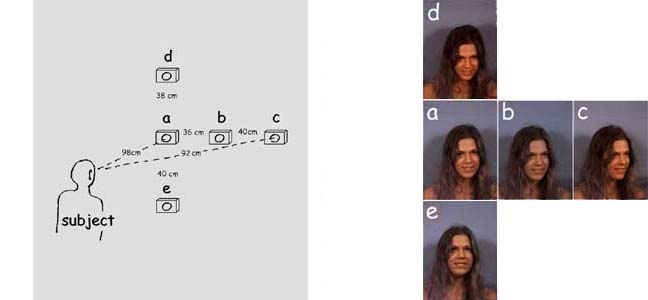
\includegraphics[width=.9\linewidth]{./images/muct-views-lores.jpg}
\end{center}

Each picture is coded with 76 facial landmark like: 
\begin{center}
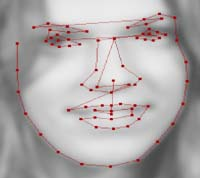
\includegraphics[width=.9\linewidth]{./images/landmarks.jpg}
\end{center}


The dataset is public available via github on the following link
\url{https://github.com/StephenMilborrow/muct}

\subsection{Solution and road map}
\label{sec:orgb19ef59}

To solve such a problem i will begin from the point of training my own model 
using Convolutional Neural Networks and compare the results by using transfer
learning from other models inception v3 , resnet, etc.

The main idea here is to create a model with 152 regression outputs giving
the respective X and Y of each point.

In case the transfer learning don't give good results another approach would
be go up on the pre-trained model and get more fine tuning.
By using the option:

\begin{verbatim}
include_top=True
\end{verbatim}

when importing the pre-trained model in Keras, and by freezing different parts
of the model is possible to archive diferent results.



\subsection{Evaluation and Metrics}
\label{sec:orgb456879}

As the problem consists on a regression model i believe that for the
evaluation of the results we could use the accuracy calculated by using one
of the regression functions R-squared OR mean-squared. 



\bibliographystyle{unsrt}
\bibliography{repport}
\end{document}